\documentclass[12pt,a4paper]{article}

\usepackage[margin=1in]{geometry}
\usepackage{amsmath, amssymb, amsthm}
\usepackage{enumitem}
\usepackage{booktabs}
\usepackage{tikz}
\usetikzlibrary{arrows.meta, positioning}

\setlength{\parindent}{0pt}
\setlength{\parskip}{6pt}

\newtheoremstyle{notestyle}
  {8pt}
  {8pt}
  {\normalfont}
  {}
  {\bfseries}
  {.}
  {0.5em}
  {}

\theoremstyle{notestyle}
\newtheorem{definition}{Definition}
\newtheorem{example}{Example}

\newenvironment{answer}
{\par\textbf{Answer.}\ }
{\hfill$\square$\par}

\newcommand{\Prob}{\mathbb{P}}

\title{\textbf{Clarification: Meaning of the $n$-Step Transition Matrix}}
\author{MA4034: Time Series and Stochastic Processes}
\date{}

\begin{document}
\maketitle

\section{What is the One-Step Transition Matrix?}

The transition matrix
\[
P=(p_{ij})
\]
tells us what can happen after \textbf{one step}.

The entry
\[
p_{ij}
\]
means
\[
\Prob(X_{n+1}=j\mid X_n=i).
\]

In words:

\[
p_{ij}=\text{probability of moving from state }i\text{ to state }j\text{ in one step}.
\]

\section{What is the $n$-Step Transition Matrix?}

The $n$-step transition matrix is
\[
P^n.
\]

The entry in row $i$, column $j$ of $P^n$ is written
\[
p_{ij}^{(n)}.
\]

It means
\[
p_{ij}^{(n)}
=
\Prob(X_n=j\mid X_0=i).
\]

In words:

\[
p_{ij}^{(n)}
=
\text{probability of being in state }j\text{ after }n\text{ steps, starting from state }i.
\]

\section{Why Do We Find $P^n$?}

We find $P^n$ because the one-step matrix only tells us what happens immediately. But often we want to know what happens after several time steps.

\[
\begin{array}{c|c}
\text{Matrix} & \text{Meaning}\\
\hline
P & \text{probabilities after 1 step}\\
P^2 & \text{probabilities after 2 steps}\\
P^3 & \text{probabilities after 3 steps}\\
P^n & \text{probabilities after }n\text{ steps}
\end{array}
\]

\textbf{Simple analogy.} If $P$ tells us where a student may go after one class period, then $P^3$ tells us where the student may be after three class periods.

\section{Why Not Just Use the One-Step Matrix?}

Because the chain may pass through many possible intermediate states.

For example, to go from state $i$ to state $j$ in two steps, the chain may go through many possible states $k$:
\[
i\to k\to j.
\]

So
\[
p_{ij}^{(2)}
=
\sum_k p_{ik}p_{kj}.
\]

This is exactly matrix multiplication.

Therefore,
\[
P^2=PP.
\]

For three steps:
\[
P^3=PPP.
\]

For $n$ steps:
\[
P^n=\underbrace{P\cdot P\cdots P}_{n\text{ times}}.
\]

\section{Transition Diagram Example}

Consider a weather model with two states:
\[
S=\text{sunny},\qquad R=\text{rainy}.
\]

Suppose:
\[
\Prob(S\to S)=0.8,\qquad \Prob(S\to R)=0.2,
\]
\[
\Prob(R\to S)=0.5,\qquad \Prob(R\to R)=0.5.
\]

\begin{center}
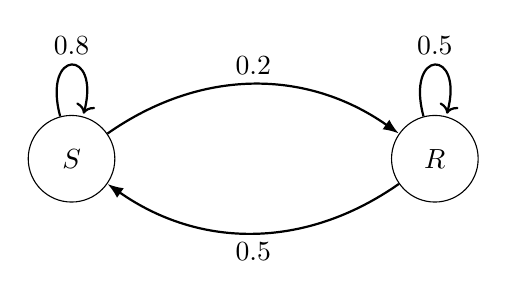
\begin{tikzpicture}[
  state/.style={circle, draw, minimum size=11mm},
  edge/.style={-{Latex[length=2mm]}, thick},
  bend angle=35
]
\node[state] (S) {$S$};
\node[state, right=35mm of S] (R) {$R$};

\draw[edge] (S) edge[loop above] node {$0.8$} (S);
\draw[edge] (R) edge[loop above] node {$0.5$} (R);
\draw[edge] (S) edge[bend left] node[above] {$0.2$} (R);
\draw[edge] (R) edge[bend left] node[below] {$0.5$} (S);
\end{tikzpicture}
\end{center}

Using state order $(S,R)$,
\[
P=
\begin{pmatrix}
0.8 & 0.2\\
0.5 & 0.5
\end{pmatrix}.
\]

\section{Worked Example 1: Two-Step Probability}

\begin{example}
If today is sunny, what is the probability that the weather is sunny after two days?
\end{example}

\begin{answer}
We need
\[
p_{SS}^{(2)}.
\]

This is the top-left entry of
\[
P^2.
\]

Compute:
\[
P^2=
\begin{pmatrix}
0.8 & 0.2\\
0.5 & 0.5
\end{pmatrix}
\begin{pmatrix}
0.8 & 0.2\\
0.5 & 0.5
\end{pmatrix}.
\]

The top-left entry is
\[
p_{SS}^{(2)}
=
(0.8)(0.8)+(0.2)(0.5).
\]

So
\[
p_{SS}^{(2)}
=
0.64+0.10
=
0.74.
\]

Therefore,
\[
\boxed{\Prob(\text{sunny after two days}\mid \text{sunny today})=0.74.}
\]
\end{answer}

\section{Meaning of the Calculation}

There are two ways to be sunny after two days if today is sunny:

\[
S\to S\to S
\]
or
\[
S\to R\to S.
\]

The first path has probability
\[
(0.8)(0.8)=0.64.
\]

The second path has probability
\[
(0.2)(0.5)=0.10.
\]

Add them:
\[
0.64+0.10=0.74.
\]

So matrix multiplication is just adding probabilities over all possible paths.

\section{Worked Example 2: Three-Step Probability}

\begin{example}
If today is rainy, what is the probability that the weather is sunny after three days?
\end{example}

\begin{answer}
We need
\[
p_{RS}^{(3)}.
\]

This is the row $R$, column $S$ entry of
\[
P^3.
\]

First compute
\[
P^2=
\begin{pmatrix}
0.74 & 0.26\\
0.65 & 0.35
\end{pmatrix}.
\]

Then
\[
P^3=P^2P.
\]

So
\[
P^3=
\begin{pmatrix}
0.74 & 0.26\\
0.65 & 0.35
\end{pmatrix}
\begin{pmatrix}
0.8 & 0.2\\
0.5 & 0.5
\end{pmatrix}.
\]

The row $R$, column $S$ entry is the second row, first column:
\[
p_{RS}^{(3)}
=
(0.65)(0.8)+(0.35)(0.5).
\]

Thus,
\[
p_{RS}^{(3)}
=
0.52+0.175
=
0.695.
\]

Therefore,
\[
\boxed{\Prob(\text{sunny after three days}\mid \text{rainy today})=0.695.}
\]
\end{answer}

\section{Long-Run Meaning of $P^n$}

Sometimes we are interested in what happens when
\[
n\to\infty.
\]

Then we study
\[
\lim_{n\to\infty}P^n.
\]

This tells us the long-run probabilities.

If the Markov chain is ergodic, then
\[
\lim_{n\to\infty}P^n
\]
has every row equal to the stationary distribution $\pi$.

That means the chain eventually forgets where it started.

\section{Worked Example 3: Long-Run Meaning}

\begin{example}
Suppose a Markov chain has stationary distribution
\[
\pi=(0.7,0.3)
\]
and is ergodic. What is
\[
\lim_{n\to\infty}P^n?
\]
\end{example}

\begin{answer}
For an ergodic Markov chain, every row of the limiting matrix is equal to the stationary distribution.

Therefore,
\[
\lim_{n\to\infty}P^n
=
\begin{pmatrix}
0.7 & 0.3\\
0.7 & 0.3
\end{pmatrix}.
\]

This means that in the long run:
\[
\Prob(\text{state 0})=0.7,
\]
and
\[
\Prob(\text{state 1})=0.3,
\]
regardless of the starting state.
\end{answer}

\section{Common Types of Questions}

\[
\begin{array}{c|c}
\text{Question asks} & \text{Use}\\
\hline
\text{after 1 step} & P\\
\text{after 2 steps} & P^2\\
\text{after 3 steps} & P^3\\
\text{after }n\text{ steps} & P^n\\
\text{long-run probability} & \lim_{n\to\infty}P^n\\
\text{stationary long-run proportion} & \pi P=\pi
\end{array}
\]

\section{Practice Questions}

\begin{enumerate}[label=\textbf{Q\arabic*.}, leftmargin=1.2cm]
    \item In words, what does $p_{ij}^{(n)}$ mean?

    \item If
    \[
    P=
    \begin{pmatrix}
    0.6 & 0.4\\
    0.3 & 0.7
    \end{pmatrix},
    \]
    find $p_{00}^{(2)}$.

    \item For the same matrix, find $p_{01}^{(2)}$.

    \item For the same matrix, if the chain starts in state 1, what is the probability it is in state 0 after two steps?

    \item Explain why matrix multiplication appears when finding two-step probabilities.

    \item Suppose
    \[
    \lim_{n\to\infty}P^n=
    \begin{pmatrix}
    0.2 & 0.8\\
    0.2 & 0.8
    \end{pmatrix}.
    \]
    What is the long-run probability of state 1?

    \item If a question asks ``What is the probability after 5 time periods?'', what matrix should you use?
\end{enumerate}

\section{Answers}

\subsection*{Answer 1}

\[
p_{ij}^{(n)}
\]
means the probability that the chain is in state $j$ after $n$ steps, given that it started in state $i$.

Mathematically,
\[
p_{ij}^{(n)}=\Prob(X_n=j\mid X_0=i).
\]

\subsection*{Answer 2}

\[
p_{00}^{(2)}
=(0.6)(0.6)+(0.4)(0.3).
\]

So
\[
p_{00}^{(2)}=0.36+0.12=0.48.
\]

\subsection*{Answer 3}

\[
p_{01}^{(2)}
=(0.6)(0.4)+(0.4)(0.7).
\]

So
\[
p_{01}^{(2)}=0.24+0.28=0.52.
\]

\subsection*{Answer 4}

Starting in state 1 and ending in state 0 after two steps is
\[
p_{10}^{(2)}.
\]

Compute:
\[
p_{10}^{(2)}
=(0.3)(0.6)+(0.7)(0.3).
\]

So
\[
p_{10}^{(2)}=0.18+0.21=0.39.
\]

\subsection*{Answer 5}

To go from state $i$ to state $j$ in two steps, the chain may pass through any intermediate state $k$:
\[
i\to k\to j.
\]

For each possible $k$, we multiply the path probabilities:
\[
p_{ik}p_{kj}.
\]

Then we add over all possible intermediate states:
\[
p_{ij}^{(2)}=\sum_k p_{ik}p_{kj}.
\]

This is exactly the rule for matrix multiplication.

\subsection*{Answer 6}

The limiting matrix is
\[
\begin{pmatrix}
0.2 & 0.8\\
0.2 & 0.8
\end{pmatrix}.
\]

The probability of state 1 is the second column:
\[
\boxed{0.8.}
\]

\subsection*{Answer 7}

If the question asks for the probability after 5 time periods, use
\[
P^5.
\]

\end{document}
